\documentclass[12pt]{beamer}
\usetheme{Warsaw}
\usepackage[utf8]{inputenc}
\usepackage{amsmath}
\usepackage{amsfonts}
\usepackage{amssymb}
\usepackage{graphicx}
\usepackage[font=Times,timeinterval=1,timeduration=2.0,timedeath=0,fillcolorwarningsecond=white!60!yellow,timewarningfirst=50,timewarningsecond=80,resetatpages=2]{tdclock}
\usepackage{tabularx}
\usepackage{array}
\usepackage{multicol}
\usepackage{longtable}
\usepackage{xcolor}
\usepackage{gensymb}
\usepackage{pgfplots}

\newcolumntype{Y}{>{\centering\arraybackslash}X}
\begin{document}
\begin{frame}
	\frametitle{Bellwork 8/16 (5 Minutes)}
	\initclock
	\textbf{[Trigonometry]}\vspace{.2cm}\\
	\vspace*{\fill}
	Let $f(x) = \sin(2x)$\\
	\vspace*{\fill}
	Evaluate: \[f\left(\frac{3\pi}{8}\right),\quad f(405\degree),\quad f\left(\frac{5\pi}{6}\right)\]\\
	\vspace*{\fill}
	\vspace*{\fill}
	\vspace*{\fill}
	\vspace*{\fill}
	\vspace*{\fill}
	\vspace*{\fill}
	\crono
	\resetcrono{\beamerbutton{reset}}
\end{frame}
\begin{frame}
	\frametitle{Exercise}
	\vspace*{\fill}
	\vspace*{\fill}
	\initclock
	$f(x) = 3x^2+8x+1$ and $h\neq0$\\
	\vspace*{\fill}
	\vspace*{\fill}
	Evaluate: \[\frac{f(a+h)-f(a)}{h}\]\\
	\vspace*{\fill}
	\vspace*{\fill}
	\vspace*{\fill}
	\vspace*{\fill}
	\crono
	\resetcrono{\beamerbutton{reset}}
\end{frame}
\begin{frame}
	\frametitle{Exercise}
	\vspace*{\fill}
	\vspace*{\fill}
	\begin{minipage}{.5\textwidth}
		$
			f(x) =
			\begin{cases}
				x+2 & x \leq 0\\
				-\frac{1}{2}x+2 & x>0
			\end{cases}
		$
	\end{minipage}%
	\begin{minipage}{.5\textwidth}
		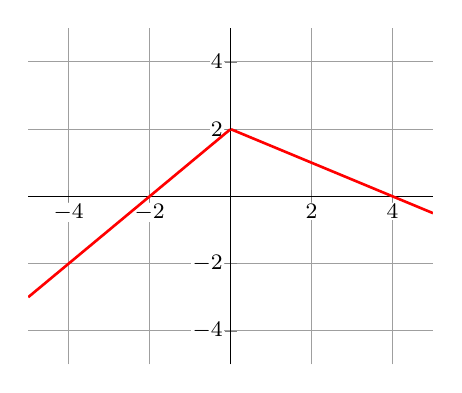
\begin{tikzpicture}[declare function={g(\x)=\x<0 ? x+2 : (\x>0 ? -0.5*x+2 : inf);}]
			\begin{axis}[unbounded coords=jump,
					grid=both,
					grid style={line width=0.35pt, draw=gray!75},
					axis lines=center,
					axis line style={-},
					xmin=-5, xmax=5,
					ymin=-5, ymax=5,
					ticklabel style={font=\footnotesize,inner sep=0.5pt,fill=white,opacity=1.0, text opacity=1},
					every axis plot/.append style={line width=0.95pt, color=red, samples=500},
					scale=0.75
				]
				\addplot[samples at={-5,-0.01,0,0.01,5}] {g(x)};
			\end{axis}
		\end{tikzpicture}
	\end{minipage}
	\vspace*{\fill}
	\begin{center}
		Evaluate: $f(-3), f(-2), f(2), f(0)$\\
	\end{center}
	\vspace*{\fill}
	\vspace*{\fill}
	\crono
	\resetcrono{\beamerbutton{reset}}
\end{frame}
\end{document}